
\chapter{Coherence for Monoidal Categories}
\lbl{app:unbiased}%
%
\index{Sigma-monoidal category@$\Sigma$-monoidal category|(}%
%
\index{monoidal category!Sigma-@$\Sigma$-|(}%
%
\index{coherence!monoidal categories@for monoidal categories|(}
%


\noindent
Here we prove the `descriptive' coherence theorems for unbiased and
classical monoidal categories and functors
(\ref{thm:diag-coh-umc},~\ref{thm:diag-coh-mc}).

Unbiased and classical monoidal categories were defined
concretely~(\ref{defn:mon-cat},~\ref{defn:lax-mon-cat}), whereas
$\Sigma$-monoidal categories were defined
abstractly~(\ref{defn:Sigma-mon-cat}).  To carry out the comparisons, we
put the definition of $\Sigma$-monoidal category into concrete terms.  Let
$\Sigma \in \Set^\nat$.  Unwinding the abstract definition, we find that a
$\Sigma$-monoidal category is a triple $A = (A, \otimes, \delta)$%
% 
\glo{cohdelta}
% 
consisting of
%
\begin{itemize}
\item a small category $A$
\item a functor $\otimes_\tau: A^n \go A$%
% 
\glo{otimestree}
%  
for each $n\in\nat$,
$\tau\in (F\Sigma)(n)$
\item an isomorphism
\[
(\delta_{\tau, \tau'})_{a_1, \ldots, a_n}:
\otimes_\tau(a_1, \ldots, a_n)
\goiso
\otimes_{\tau'}(a_1, \ldots, a_n)
\]
in $A$ for each $n\in\nat, \tau, \tau' \in (F\Sigma)(n), a_i \in A$
(usually just written $\delta_{\tau, \tau'}$)
\end{itemize}
%
satisfying 
%
\begin{description}
\item[\astyle{MC1}]	% \lbl{ax:obj:nat}
$(\delta_{\tau, \tau'})_{a_1, \ldots, a_n}$ is natural in $a_1,
\ldots, a_n \in A$, for each $n\in\nat, \tau, \tau' \in (F\Sigma)(n)$
\item[\astyle{MC2}] 	% \lbl{ax:obj:func}
$\delta_{\tau', \tau''} \of \delta_{\tau, \tau'} = \delta_{\tau, \tau''}$
and $1 = \delta_{\tau, \tau}$, for all $n\in\nat, \tau, \tau', \tau'' \in
(F\Sigma)(n)$
\item[\astyle{MC3}]	% \lbl{ax:obj:alg-obj}
$\otimes_{\tau \sof (\tau_1, \ldots, \tau_n)} = (A^{k_1 + \cdots + k_n}
\goby{\otimes_{\tau_1} \times\cdots\times \otimes_{\tau_n}} A^n
\goby{\otimes_\tau} A)$ for all $n, k_i \in\nat, \tau\in (F\Sigma)(n),
\tau_i \in (F\Sigma)(k_i)$; and $1_A = \otimes_\utree$
% 
\item[\astyle{MC4}] 	% \lbl{ax:obj:alg-map}
the diagram
%
\begin{diagram}[width=2em]
\begin{array}[t]{l}
\otimes_\tau ( \otimes_{\tau_1}(a_1^1, \ldots, a_1^{k_1}), \ldots, \\
\otimes_{\tau_n}(a_n^1, \ldots, a_n^{k_n}))			
\end{array}
&
\rEquals							&
\otimes_{\tau\sof(\tau_1, \ldots, \tau_n)} ( a_1^1, \ldots, a_n^{k_n})	\\
\dTo<{\otimes_\tau(\delta_{\tau_1,\tau'_1}, \ldots, 
\delta_{\tau_n,\tau'_n})}					&
								&
									\\
\begin{array}{l}
\otimes_\tau ( \otimes_{\tau'_1}(a_1^1, \ldots, a_1^{k_1}), \ldots, \\
\otimes_{\tau'_n}(a_n^1, \ldots, a_n^{k_n}))			
\end{array}
&
								&
\dTo>{\delta_{\tau\sof(\tau_1, \ldots, \tau_n), 
\tau'\sof(\tau'_1, \ldots, \tau'_n)}}					\\
\dTo<{\delta_{\tau,\tau'}}					&
								&
									\\
\begin{array}[b]{l}
\otimes_{\tau'} ( \otimes_{\tau'_1}(a_1^1, \ldots, a_1^{k_1}), \ldots, \\
\otimes_{\tau'_n}(a_n^1, \ldots, a_n^{k_n}))			
\end{array}
&
\rEquals							&
\otimes_{\tau'\sof(\tau'_1, \ldots, \tau'_n)} ( a_1^1, \ldots, a_n^{k_n})\\
\end{diagram}
%
commutes, for all $n, k_i \in\nat, \tau,\tau'\in (F\Sigma)(n),
\tau_i,\tau'_i\in (F\Sigma)(k_i), a_i^j\in A$.
\end{description}
%
A lax monoidal functor $(P, \pi): (A,\otimes,\delta) \go
(A',\otimes,\delta)$ (where, in an abuse of notation, we write
$\otimes$ for the tensor and $\delta$ for the coherence maps in both $A$
and $A'$) consists of
%
\begin{itemize}
\item a functor $P: A \go A'$
\item a map
\[
(\pi_\tau)_{a_1, \ldots, a_n}:
\otimes_\tau(Pa_1, \ldots, Pa_n) \go P\otimes_\tau (a_1, \ldots, a_n)
\]
(usually just written $\pi_\tau$) for each $n\in\nat, \tau\in (F\Sigma)(n),
a_i\in A$ 
\end{itemize}
%
satisfying
%
\begin{description}
\item[\astyle{MF1}] 	% \lbl{ax:map:nat}
$(\pi_\tau)_{a_1, \ldots, a_n}$ is natural in $a_1, \ldots, a_n \in A$
\item[\astyle{MF2}]	% \lbl{ax:map:nat-tau}
the diagram
%
\begin{diagram}[size=2em]
\otimes_\tau (Pa_1, \ldots, Pa_n)	&
\rTo^{\delta_{\tau,\tau'}}		&
\otimes_{\tau'}(Pa_1, \ldots, Pa_n)	\\
\dTo<{\pi_\tau}				&
					&
\dTo>{\pi_{\tau'}}			\\
P\otimes_\tau (a_1, \ldots, a_n)	&
\rTo_{P\delta_{\tau,\tau'}}		&
P\otimes_{\tau'} (a_1, \ldots, a_n)	\\
\end{diagram}
%
commutes, for all $n\in\nat, \tau,\tau'\in (F\Sigma)(n), a_i\in A$
\item[\astyle{MF3}] 	% \lbl{ax:map:coh}
the diagram
%
\begin{diagram}[width=2em]
\begin{array}[t]{l}
\otimes_\tau (\otimes_{\tau_1} (Pa_1^1, \ldots, Pa_1^{k_1}), \ldots,\\
\otimes_{\tau_n} (Pa_n^1, \ldots, Pa_n^{k_n}))		
\end{array}
&
\rEquals						&
\otimes_{\tau\sof(\tau_1, \ldots, \tau_n)} (Pa_1^1, \ldots, Pa_n^{k_n})	\\
\dTo<{\otimes_\tau (\pi_{\tau_1}, \ldots, \pi_{\tau_n})}&
							&
							\\
\begin{array}{l}
\otimes_\tau ( P\otimes_{\tau_1}(a_1^1, \ldots, a_1^{k_1}), \ldots,\\
P\otimes_{\tau_n}(a_n^1, \ldots, a_n^{k_n}) )		
\end{array}
&
							&
\dTo>{\pi_{\tau\sof(\tau_1, \ldots, \tau_n)}}		\\
\dTo<{\pi_\tau}						&
							&
							\\
\begin{array}[b]{l}
P\otimes_\tau (\otimes_{\tau_1}(a_1^1, \ldots, a_1^{k_1}), \ldots,\\
\otimes_{\tau_n}(a_n^1, \ldots, a_n^{k_n}))		
\end{array}
&
\rEquals						&
P\otimes_{\tau\sof(\tau_1, \ldots, \tau_n)} (a_1^1, \ldots, a_n^{k_n})\\
\end{diagram}
%
commutes for all $n, k_i\in\nat, \tau\in (F\Sigma)(n), \tau_i\in
(F\Sigma)(k_i), a_i^j\in A$, and the diagram
%
\begin{diagram}[size=2em]
Pa	&\rEquals	&\otimes_\utree Pa	\\
\dTo<1	&		&\dTo>{\pi_1}		\\
Pa	&\rEquals	&P\otimes_\utree a	\\
\end{diagram}
% 
commutes for all $a\in A$ (where in the expression `$\pi_1$', the $1$ is
the unit of the operad $F\Sigma$).
\end{description}
%
A weak (respectively, strict) monoidal functor is a lax monoidal functor
$(P, \pi)$ in which all the $\pi_\tau$'s are isomorphisms (respectively,
identities).  

In the cases at hand, the object $\Sigma$ of $\Set^\nat$ is either the
terminal object $1$ (for unbiased monoidal categories) or the object
$\Sigma_\mr{c}$ defined in Theorem~\ref{thm:diag-coh-mc} (for classical
monoidal categories).  The \Set-operad $F\Sigma$ is then, respectively,
either the operad $\tr$ of all trees~(\ref{eg:opd-of-trees}) or the operad
$\ctr$ of classical trees~(\ref{eg:opd-of-cl-trees}).

Sections~\ref{sec:app-UMC} and~\ref{sec:app-MC} prove coherence for
unbiased and classical monoidal categories, respectively.  The unbiased
case contains some scary-looking expressions but is completely
straightforward: one only needs to be awake, not clever.  By contrast, the
classical case requires guile, cunning and trickery---attributes not
displayed here, but vital to the proofs of the coherence theorems upon
which we rely.

All of the results that we prove continue to hold in the more general
setting of $\Sigma$-bicategories~(\ref{sec:notions-bicat}).%
%
\index{bicategory!Sigma-@$\Sigma$-}%
%
\index{Sigma-bicategory@$\Sigma$-bicategory}
%
%
 The proofs
need only superficial changes of the kind described
in~\ref{sec:notions-bicat}; for instance, the category $A$ becomes a
\Cat-graph $B$ and tensor becomes composition.





\section{Unbiased monoidal categories}
\lbl{sec:app-UMC}%
%
\index{monoidal category!unbiased|(}
%

The plan is to define a functor
\[
J: 1\hyph\MClax \go \UMClax,
\]
to prove that it is an isomorphism (by showing in turn that it is injective
on objects, surjective on objects, faithful, and full), and then to prove
that it restricts to isomorphisms
\[
1\hyph\MCwk \goiso \UMCwk,
\diagspace
1\hyph\MCstr \goiso \UMCstr
\]
at the weak and strict levels.

%
\index{tree|(}
%
Recall from~\ref{eg:opd-of-trees} that $\utree\in\tr(1)$ denotes
the `null' or identity tree, and that $\nu_n \in \tr(n)$ denotes the
simplest $n$-leafed tree 
% \drmk{pic of corolla}.  
$\begin{centredpic}
\begin{picture}(3,2)(-1.5,0)
% lower layer
\put(0,0){\line(0,1){1}}
\cell{0}{1}{c}{\vx}
% upper layer
\put(0,1){\line(-3,2){1.5}}
\cell{0}{1.8}{c}{\cdots}
\put(0,1){\line(3,2){1.5}}
\end{picture}
\end{centredpic}$.
% 
(Recall also that $\nu_1 =
\setlength{\unitlength}{1em}
\begin{array}{c}
\begin{picture}(0,2)(0,0)
\put(0,0){\line(0,1){1}}
\cell{0}{1}{c}{\vx}
\put(0,1){\line(0,1){1}}
\end{picture}
\end{array}
% 
\neq
% 
\setlength{\unitlength}{1em}
\begin{array}{c}
\begin{picture}(0,1)(0,0)
\put(0,0){\line(0,1){1}}
\end{picture}
\end{array}$.) 
We will be composing trees---that is, composing in the operad $\tr$---and
in particular we will often use the composite tree
% 
\[
\nu_n \of (\nu_{k_1}, \ldots, \nu_{k_n}) = 
% \drmk{picture}.
\begin{centredpic}
\begin{picture}(6,3)(-3,0)
% bottom layer
\put(0,0){\line(0,1){1}}
% middle layer
\cell{0}{1}{c}{\vx}
\put(0,1){\line(-2,1){2}}
\put(0,1){\line(2,1){2}}
\cell{0}{1.8}{c}{\cdots}
% top layer
\cell{-2}{2}{c}{\vx}
\put(-2,2){\line(-1,1){1}}
\put(-2,2){\line(1,1){1}}
\cell{-2}{2.8}{c}{\cdots}
\cell{2}{2}{c}{\vx}
\put(2,2){\line(-1,1){1}}
\put(2,2){\line(1,1){1}}
\cell{2}{2.8}{c}{\cdots}
\end{picture}
\end{centredpic}.
% \dr{36}{18}.
\]

Our first task is to define a functor $J: 1\hyph\MClax \go \UMClax$.
%
\begin{description}
\item[On objects] Let $(A, \otimes, \delta)$ be an object of
$1\hyph\MClax$.  The unbiased monoidal category $J(A, \otimes, \delta)$ is
given by taking the underlying category to be $A$, the $n$-fold tensor
$\otimes_n: A^n \go A$ to be $\otimes_{\nu_n}$, and the coherence maps to
be
%
\begin{eqnarray*}
\lefteqn{\gamma_{((a_1^1, \ldots, a_1^{k_1}), \ldots, (a_n^1, \ldots, a_n^{k_n}))}
=
(\delta_{\nu_n \sof (\nu_{k_1}, \ldots, \nu_{k_n}), 
\nu_{k_1 + \cdots + k_n}})_{a_1^1, \ldots, a_n^{k_n}}:}	\\
&((a_1^1 \otimes\cdots\otimes a_1^{k_1}) \otimes\cdots\otimes
(a_n^1 \otimes\cdots\otimes a_n^{k_n}))
\go
(a_1^1 \otimes\cdots\otimes a_n^{k_n})
\end{eqnarray*}
% 
and
\[
\iota_a = (\delta_{\utree, \nu_1})_a: a \go (a).
\]
%
\item[On maps] Let $(P, \pi): A \go A'$ be a map in $1\hyph\MClax$.  The
lax monoidal functor $J(P, \pi): J(A) \go J(A')$ is given by taking the
same underlying functor $P$, and by taking the coherence map
\[
\pi_{a_1, \ldots, a_n}:
(Pa_1 \otimes \cdots \otimes Pa_n) 
\go
P(a_1 \otimes\cdots\otimes a_n)
\]
(re-using the letter $\pi$, in another slight abuse) to be
$(\pi_{\nu_n})_{a_1, \ldots, a_n}$. 
\end{description}

\begin{lemma}
This defines a functor $J: 1\hyph\MClax \go \UMClax$.
\end{lemma}

\begin{proof} 
We have to check three things:
%
\begin{itemize}
\item $J(A,\otimes,\delta)$ as defined above really is an unbiased
monoidal category---in other words, the axioms in
Definition~\ref{defn:lax-mon-cat} hold.  Naturality and invertibility of
$\gamma$ and $\iota$  follow from the same properties for $\delta$. The
associativity axiom holds because both routes around the square are
\[
(\delta_{ \nu_n\sof (\nu_{m_1}, \ldots, \nu_{m_n}) \sof (\nu_{k_1^1},
\ldots, \nu_{k_n^{m_n}}), \nu_{k_1^1 + \cdots + k_n^{m_n}}})_%
{a_{1,1,1}, \ldots, a_{n,m_n,k_n^{m_n}}},
\]
as can be shown from axioms~\astyle{MC2} and~\astyle{MC4}.  The identity
axioms hold by similar reasoning.
\item $J(P, \pi)$ as defined above really is a lax monoidal functor between
unbiased monoidal categories (Definition~\ref{defn:u-lax-mon-ftr}).
Naturality of $\pi_{a_1, \ldots, a_n}$ in the $a_i$'s follows from the same
naturality for $\pi_{\nu_n}$.  The coherence axioms can be deduced from
axioms \astyle{MF1}--\astyle{MF3}.
\item $J$ preserves composition and identities.  This is trivial.
\done
\end{itemize}
\end{proof}

\begin{lemma}	\lbl{lemma:u-inj}
The functor $J: 1\hyph\MClax \go \UMClax$ is injective on objects.
\end{lemma}

\begin{proof}
Suppose that $(A, \otimes, \delta)$ and $(A', \otimes', \delta')$ are
$1$-monoidal categories with $J(A, \otimes, \delta) = J(A', \otimes',
\delta')$.  (Just for once, the tensor of $A'$ is written $\otimes'$ rather
than $\otimes$, and similarly $\delta'$ rather than $\delta$.)  Then:
%
\begin{itemize}
\item $A = A'$ immediately.
\item $\otimes_\tau = \otimes'_\tau$ for all $n\in\nat$ and
$\tau\in\tr(n)$.  This is proved by induction on $\tau$, using the
description of $\tr$ in~\ref{eg:opd-of-trees}.  Since there will be many
inductions on trees in this appendix, I will write this one out in full and
leave the others to the virtuous reader.  First, $\otimes_\utree = 1_A =
\otimes'_\utree$ by~\astyle{MC3}.  Second, take $\tau_1\in\tr(k_1), \ldots,
\tau_n\in\tr(k_n)$. Then
%
\begin{eqnarray*}
\otimes_{(\tau_1, \ldots, \tau_n)}	&=	&
\otimes_{\nu_n \sof (\tau_1, \ldots, \tau_n)}	\\
&=&\otimes_{\nu_n} \of (\otimes_{\tau_1} \times\cdots\times
\otimes_{\tau_n}),   
\end{eqnarray*}
%
again by~\astyle{MC3}.  But $\otimes_{\nu_n} = \otimes'_{\nu_n}$ since
$J(A, \otimes, \delta) = J(A', \otimes', \delta')$, and $\otimes_{\tau_i} =
\otimes'_{\tau_i}$ by inductive hypothesis, so $\otimes_{(\tau_1, \ldots,
\tau_n)} = \otimes'_{(\tau_1, \ldots, \tau_n)}$, completing the induction.
\item $\delta_{\tau,\tau'} = \delta'_{\tau,\tau'}$ for all $\tau, \tau' \in
\tr(n)$.  Since $\delta_{\tau,\tau'} = \delta_{\tau',\nu_n}^{-1} \of
\delta_{\tau,\nu_n}$, it is enough to prove this in the case
$\tau'=\nu_n$; and that is done by another short induction on $\tau$.
\done
\end{itemize}
\end{proof}

\begin{lemma}
The functor $J: 1\hyph\MClax \go \UMClax$ is surjective on objects.
\end{lemma}

\begin{proof}
Take an unbiased monoidal category $(A, \otimes, \gamma, \iota)$.  Attempt
to define a $1$-monoidal category $(A, \otimes, \delta)$ as follows:
%
\begin{itemize}
\item The underlying category $A$ is the same.
\item The tensor $\otimes_\tau: A^n \go A$, for $\tau\in\tr(n)$, is defined
inductively on $\tau$ by $\otimes_\utree = 1_A$ and 
\[
\otimes_{(\tau_1, \ldots, \tau_n)} = 
(A^{k_1 + \cdots + k_n} 
\goby{\otimes_{\tau_1} \times\cdots\times \otimes_{\tau_n}}
A^n \goby{\otimes_n} A).
\]
\item The coherence isomorphisms are defined by $\delta_{\tau, \tau'} =
\delta_{\tau'}^{-1} \of \delta_\tau$, where in turn
\[
\delta_\tau: \otimes_\tau(a_1, \ldots, a_n) \goiso 
(a_1 \otimes\cdots\otimes a_n)
\]
is defined by taking $\delta_\utree = \iota$ and taking $\delta_{(\tau_1,
\ldots, \tau_n)}$ to be the composite
%
\begin{eqnarray*}
&&
(\otimes_{\tau_1}(a_1^1, \ldots, a_1^{k_1}) 
\ \otimes\ \cdots\ \otimes\ 
\otimes_{\tau_n}(a_n^1, \ldots, a_n^{k_n}) )	\\ &
\goby{(\delta_{\tau_1} \otimes\cdots\otimes \delta_{\tau_n})} &	
((a_1^1 \otimes\cdots\otimes a_1^{k_1}) \otimes\cdots\otimes
(a_n^1 \otimes\cdots\otimes a_n^{k_n}))		\\
&
\goby{\gamma}	&	
(a_1^1 \otimes\cdots\otimes a_n^{k_n}).
\end{eqnarray*}
%
\end{itemize}
% 
This does indeed satisfy the axioms for a $1$-monoidal category:
%
\begin{description}
\item[\astyle{MC1}, \astyle{MC2}] Immediate.
\item[\astyle{MC3}] That $\otimes_\utree = 1_A$ is immediate.  The other
equation can be proved by induction on $\tau$, or by using the fact that
$\tr$ is the free operad on $1 \in\Set^\nat$ and that
$(\Cat(A^n,A))_{n\in\nat}$ forms an operad.
\item[\astyle{MC4}] It is enough to show that this axiom is satisfied when
$\tau'=\nu_n, \tau'_1=\nu_{k_1}, \ldots, \tau'_n=\nu_{k_n}$: in other
words, that
%
\begin{diagram}[width=2em]
\begin{array}[t]{l}
\otimes_\tau ( \otimes_{\tau_1}(a_1^1, \ldots, a_1^{k_1}), \ldots, \\
\otimes_{\tau_n}(a_n^1, \ldots, a_n^{k_n}))			
\end{array}
&
\rEquals							&
\otimes_{\tau\sof(\tau_1, \ldots, \tau_n)} ( a_1^1, \ldots, a_n^{k_n})	\\
\dTo<{\otimes_\tau(\delta_{\tau_1}, \ldots, 
\delta_{\tau_n})}						&
								&
\dTo>{\delta_{\tau\sof(\tau_1,\ldots,\tau_n)}}				\\
\begin{array}{l}
\otimes_\tau ( (a_1^1 \otimes\cdots\otimes a_1^{k_1})
\otimes\cdots	\\
\otimes (a_n^1 \otimes\cdots\otimes a_n^{k_n}) )
\end{array}
&
								&
(a_1^1 \otimes\cdots\otimes a_n^{k_n})					\\
\dTo<{\delta_\tau}						&
								&
\uTo>{\delta_{\nu_n \sof (\nu_{k_1},\ldots,\nu_{k_n})} = \gamma}	\\
\begin{array}[b]{l}
((a_1^1 \otimes\cdots\otimes a_1^{k_1}) \otimes\cdots \\
\otimes (a_n^1 \otimes\cdots\otimes a_n^{k_n}))			
\end{array}
&
\rEquals							&
\begin{array}[b]{r}
((a_1^1 \otimes\cdots\otimes a_1^{k_1}) \otimes\cdots	\\
\otimes (a_n^1 \otimes\cdots\otimes a_n^{k_n}))				
\end{array}
\\
\end{diagram}
%
commutes.  This is done by induction on $\tau$, using the associativity
axiom for unbiased monoidal categories.
\end{description}
% 
Finally, $J(A,\otimes,\delta) = (A,\otimes,\gamma,\iota)$:
%
\begin{itemize}
\item Clearly the underlying categories agree, both being $A$.
\item We have 
\[
\otimes_{\nu_n} 
= \otimes_{(\utree, \ldots, \utree)} 
= \otimes_n \of (\otimes_\utree \times\cdots\times \otimes_\utree)
= \otimes_n,
\]
so the tensor products agree.
\item Certainly $\delta_\utree = \iota$.  Also
\[
\delta_{\nu_k} 
= \gamma \of (\delta_\utree \otimes\cdots\otimes \delta_\utree)
= \gamma \of (\iota \otimes\cdots\otimes \iota)
= 1
\]
for any $k$, so 
\[
\delta_{\nu_n \sof (\nu_{k_1}, \ldots, \nu_{k_n})} 
= \gamma \of (\delta_{\nu_{k_1}} \otimes\cdots\otimes \delta_{\nu_{k_n}})
= \gamma.
\]
Hence the coherence maps $\iota$ and $\gamma$ also agree.
\done
\end{itemize}
\end{proof}

\begin{lemma}
The functor $J: 1\hyph\MClax \go \UMClax$ is faithful.
\end{lemma}

\begin{proof}
Suppose that $A \parpair{(P,\pi)}{(Q,\chi)} A'$ in $1\hyph\MClax$ with
$J(P,\pi) = J(Q,\chi)$.  Then:
%
\begin{itemize}
\item $P=Q$ immediately.
\item $\pi_\tau = \chi_\tau$ for all $\tau\in\tr(n)$, by an induction on
$\tau$ similar to the one written out in the proof of~\ref{lemma:u-inj}.
\done
\end{itemize}
\end{proof}

\begin{lemma}	\lbl{lemma:u-full}
The functor $J: 1\hyph\MClax \go \UMClax$ is full.
\end{lemma}

\begin{proof}
Let $A, A' \in 1\hyph\MClax$ and let $J(A) \goby{(P,\pi)} J(A')$ be a map
in $\UMClax$.  Attempt to define a map $A \goby{(P,\pi)} A'$ in
$1\hyph\MClax$ (where as usual we abuse notation by recycling the name
$(P,\pi)$) as follows:
%
\begin{itemize}
\item The underlying functor $P$ is the same.
\item The coherence maps $\pi_\tau$ are defined by induction on $\tau$.  We
take $\pi_\utree = 1$ and take
\[
\otimes_{(\tau_1, \ldots, \tau_n)} (Pa_1^1, \ldots, Pa_n^{k_n}) 
\goby{\pi_{(\tau_1, \ldots, \tau_n)}}
P\otimes_{(\tau_1, \ldots, \tau_n)} (a_1^1, \ldots, a_n^{k_n}) 
\]
to be the composite
%
\begin{eqnarray*}
\lefteqn{
(\otimes_{\tau_1}(Pa_1^1, \ldots, Pa_1^{k_1}) 
\ \otimes\ \cdots\ \otimes\ 
\otimes_{\tau_n}(Pa_n^1, \ldots, Pa_n^{k_n}) )}	\\ 
&
\goby{(\pi_{\tau_1} \otimes\cdots\otimes \pi_{\tau_n})}	&
\begin{array}[t]{l}
(P\otimes_{\tau_1}(a_1^1, \ldots, a_1^{k_1}) \ \otimes\ \cdots\\
\otimes\ P\otimes_{\tau_n}(a_n^1, \ldots, a_n^{k_n}))	
\end{array}
\\
&
\goby{\pi_{\otimes_{\tau_1}(a_1^1, \ldots, a_1^{k_1}), \ldots,
\otimes_{\tau_n}(a_n^1, \ldots, a_n^{k_n})}}	&
P(a_1^1 \otimes\cdots\otimes a_n^{k_n}).
\end{eqnarray*}
%
\end{itemize}

This does satisfy the axioms above for a lax monoidal functor between
$1$-monoidal categories:
%
\begin{description}
\item[\astyle{MF1}] Immediate.
\item[\astyle{MF2}] It is enough to prove this when $\tau'=\nu_n$; in
other words, that
%
\begin{diagram}[size=2em]
\otimes_\tau (Pa_1, \ldots, Pa_n)	&\rTo^{\delta_\tau}	&
(Pa_1 \otimes\cdots\otimes Pa_n)	\\
\dTo<{\pi_\tau}				&			&
\dTo>{\pi_{a_1,\ldots,a_n}}		\\
P\otimes_\tau(a_1, \ldots, a_n)		&
\rTo_{P\delta_\tau}			&
P(a_1 \otimes\cdots\otimes a_n)		\\
\end{diagram}
%
commutes.  This is done by induction on $\tau$, using the coherence
axioms for lax monoidal functors between unbiased monoidal categories.
\item[\astyle{MF3}] This is, inevitably, another induction on $\tau$.
\end{description}

Finally, $J(P,\pi) = (P,\pi)$:
%
\begin{itemize}
\item The underlying functors agree, both being $P$.
\item We have
%
\begin{eqnarray*}
(\pi_{\nu_n})_{a_1, \ldots, a_n} &=	&
\pi_{\otimes_\utree(a_1), \ldots, \otimes_\utree(a_n)}
\of
((\pi_\utree)_{a_1} \otimes\cdots\otimes (\pi_\utree)_{a_n})	\\
	&=	&
\pi_{a_1, \ldots, a_n} \of (1 \otimes\cdots\otimes 1)	\\
	&=	&
\pi_{a_1, \ldots, a_n},
\end{eqnarray*}
so the coherence maps also agree.
\done
\end{itemize}
\end{proof}%
%
\index{tree|)}
%

Theorem~\ref{thm:diag-coh-umc} now follows in the lax case: $\UMClax \iso
1\hyph\MClax$.  The weak and strict cases follow from:

\begin{lemma}	\lbl{lemma:u-restrict}
The isomorphism $J: 1\hyph\MClax \goiso \UMClax$ restricts to 
isomorphisms
\[
1\hyph\MCwk \goiso \UMCwk,
\diagspace
1\hyph\MCstr \goiso \UMCstr.
\]
\end{lemma}

\begin{proof}
Trivial.
\done
\end{proof}%
%
\index{monoidal category!unbiased|)}
%




\section{Classical monoidal categories}
\lbl{sec:app-MC}%
%
\index{monoidal category!classical|(}
%

The strategy is the same as in the unbiased setting: we define
a functor
\[
J: \Sigma_\mr{c}\hyph\MClax \go \MClax,
\]
prove it is an isomorphism, then prove that it restricts to isomorphisms at
the levels of weak and strict maps.

%
\index{tree!classical|(}
%
We will use the operad \ctr\ of classical or unitrivalent
trees~(\ref{eg:opd-of-cl-trees}).  In particular, we have trees
\[
\nu_0 = \nuzeropic \in \ctr(0), 
\diagspace
\nu_2 = \nutwopic \in \ctr(2), 
\]
the identity tree $\utree\in\ctr(1)$, and composite trees
\[
\begin{array}{c}
\nu_2 \of (\nu_2, \utree) = \assleftpic \in \ctr(3),
\diagspace
\nu_2 \of (\utree, \nu_2) = \assrightpic \in \ctr(3),\\
\nu_2 \of (\nu_0, \utree) = \lambdapic \in \ctr(1),
\diagspace
\nu_2 \of (\utree, \nu_0) = \rhopic \in \ctr(1).
\end{array}
\]

To prove our result, we will certainly want to use the fact that `all
diagrams commute' in a classical monoidal category, and some similar
statement for monoidal functors.  In other words, the proof of our unified
coherence theorem for classical monoidal categories and functors will
depend on pre-established coherence theorems.  A rather vague description
of those theorems was given in~\ref{sec:mon-cats}.  Using the language of
trees we can now be more precise.

So, let $A = (A, \otimes, I, \alpha, \lambda, \rho)$ be a classical
monoidal category.  We define for each $n\in\nat$ and $\tau\in\ctr(n)$ a
functor $\otimes_\tau: A^n \go A$.  This definition is by induction on
$\tau$ (using the description of $\ctr$ in~\ref{eg:opd-of-cl-trees}), as
follows:
%
\begin{itemize}
\item $\otimes_\utree: A^1 \go A$ is the canonical isomorphism
\item $\otimes_\nuzeropic: A^0 \go A$ `is' the unit object $I$ of $A$
\item if $\tau_1\in\ctr(k_1)$ and $\tau_2\in\ctr(k_2)$ then 
$\otimes_{(\tau_1, \tau_2)}$ is the composite
\[
A^{k_1 + k_2} \goby{\otimes_{\tau_1} \times \otimes_{\tau_2}}
A^2 \goby{\otimes} A.
\]
\end{itemize}
% 
The coherence results from~\ref{sec:mon-cats} can now be stated as:
%
\begin{itemize}
\item Let $A$ be a classical monoidal category.  Then for each $n\in\nat$
and $\tau, \tau' \in \ctr(n)$, there is a unique natural transformation
$A^n \ctwomult{\otimes_\tau}{\otimes_{\tau'}}{} A$ built out of $\alpha$,
$\lambda$ and $\rho$.
\item Let $(P, \pi): A \go A'$ be a lax monoidal functor.  Then for each
$n\in\nat$ and $\tau, \tau' \in \ctr(n)$, there is a unique natural
transformation
%
\begin{diagram}
A^n		&\rTo^{\otimes_\tau}	&A		\\
\dTo<{P^n}	&\nent			&\dTo>P		\\
A'^n		&\rTo_{\otimes_{\tau'}}	&A'
\end{diagram}
%
built out of the coherence isomorphisms $\alpha, \lambda$ and $\rho$ of $A$ and
$A'$ and the coherence maps $\pi_{\dashbk,\dashbk}$ and $\pi_\cdot$.
\end{itemize}
%
I will refer to these as \demph{informal coherence}%
%
\index{coherence!monoidal categories@for monoidal categories!informal}
%
for classical monoidal
categories and functors.  They could be made precise by defining `built out
of', but I hope the reader will be content to use them in their present
imprecise form.

Our first task is to define a functor $J: \Sigma_\mr{c}\hyph\MClax \go
\MClax$.

\begin{description}
\item[On objects] Let $(A, \otimes, \delta)$ be an object of
$\Sigma_\mr{c}\hyph\MClax$, as described in the introduction to this
appendix.  Then the classical monoidal category $J(A, \otimes, \delta)$ is
given by taking the underlying category to be $A$, the tensor to be
$\otimes_\nutwopic$, the unit object to be $\otimes_\nuzeropic$, and
the coherence isomorphisms to be
\[
\alpha = \delta_{\tau_1, \tau'_1},
\diagspace
\lambda = \delta_{\tau_2, \utree},
\diagspace
\rho = \delta_{\tau_3, \utree}
\]
where
\[
\tau_1 = \assleftpic,
\diagspace
\tau'_1 = \assrightpic,
\diagspace
\tau_2 = \lambdapic,
\diagspace
\tau_3 = \rhopic.
\]
%
\item[On maps] Let $(P, \pi): A \go A'$ be a map in
$\Sigma_\mr{c}\hyph\MClax$, also as described in the introductory section.
Then the lax monoidal functor $J(P,\pi): J(A) \go J(A')$ is given by taking
the same underlying category $P$ and coherence maps
\[
\pi_{\dashbk, \dashbk} = \pi_{\nutwopic},
\diagspace
\pi_\cdot = \pi_{\nuzeropic}.
\] 
% %
\end{description}

\begin{lemma}
This defines a functor $J: \Sigma_\mr{c}\hyph\MClax \go \MClax$.
\end{lemma}

\begin{proof}
We have to check three things:
%
\begin{itemize}
\item $J(A, \otimes, \delta)$ as defined above really is a classical
monoidal category.  Naturality and invertibility of $\alpha$, $\lambda$ and
$\rho$ follow from the same properties of $\delta$.  The
pentagon~(\ref{defn:mon-cat}) commutes because each route around it is
$\delta_{\tau,\tau'}$, where
\[
\tau = 
\begin{array}{c}\epsfig{file=pentagonleftpic.eps}\end{array},
\diagspace
\tau' = 
\begin{array}{c}\epsfig{file=pentagonrightpic.eps}\end{array}.
\]
% 
Similarly, the triangle commutes because both ways round it are
$\delta_{\sigma,\sigma'}$, where
\[
\sigma = 
\begin{array}{c}\epsfig{file=trianglepic.eps}\end{array},
\diagspace
\sigma' = \nutwopic.
\]
\item $(J,\pi)$ as defined above really is a lax monoidal functor between
classical monoidal categories.  The axioms can be deduced from
\astyle{MF1}--\astyle{MF3}. 
\item $J$ preserves composition and identities.  This is trivial.%
\done
\end{itemize}
\end{proof}

\begin{lemma}	\lbl{lemma:c-inj}
The functor $J: \Sigma_\mr{c}\hyph\MClax \go \MClax$ is injective on
objects. 
\end{lemma}

\begin{proof}
Suppose that $(A, \otimes, \delta)$ and $(A', \otimes', \delta')$ are
$\Sigma_\mr{c}$-monoidal categories with $J(A, \otimes, \delta) = J(A',
\otimes', \delta')$.  Then:
%
\begin{itemize}
\item $A = A'$ immediately.
\item $\otimes_\tau = \otimes'_\tau$ for all $n\in\nat$ and
$\tau\in\tr(n)$.  This is proved by induction on $\tau$, using the
definition of $\ctr$ in~\ref{eg:opd-of-cl-trees}.  As in the previous
section, there will be many proofs by induction on the structure of a tree;
and as a sample of the technique in the classical case, I will write this
one out in full.  First, $\otimes_\utree = 1_A = \otimes'_\utree$
by~\astyle{MC3}.  Second, $\otimes_\nuzeropic = I = \otimes'_\nuzeropic$
since $J(A, \otimes, \delta) = J(A', \otimes', \delta')$.  Third, take
$\tau_1 \in \ctr(k_1)$ and $\tau_2 \in \ctr(k_2)$.  Then
\[
\otimes_{(\tau_1, \tau_2)} 
= \otimes_{\nutwopic \sof (\tau_1, \tau_2)}
= \otimes_\nutwopic \of (\otimes_{\tau_1} \times \otimes_{\tau_2}),
\]
again by~\astyle{MC3}.  But $\otimes_\nutwopic = \otimes'_\nutwopic$ since
$J(A, \otimes, \delta) = J(A', \otimes', \delta')$, and $\otimes_{\tau_i} =
\otimes'_{\tau_i}$ by inductive hypothesis, so $\otimes_{(\tau_1, \tau_2)}
= \otimes'_{(\tau_1, \tau_2)}$, completing the induction.
\item $\delta_{\tau, \tau'} = \delta'_{\tau, \tau'}$ for all $\tau, \tau'
\in \ctr(n)$.  This follows from informal coherence for classical
monoidal categories---in particular, from the fact that there is \emph{at
least} one natural transformation $\otimes_\tau \go \otimes_{\tau'}$ built
up from $\alpha$, $\lambda$ and $\rho$.  
\done
\end{itemize}
\end{proof}

\begin{lemma}
The functor $J: \Sigma_\mr{c}\hyph\MClax \go \MClax$ is surjective on
objects. 
\end{lemma}

\begin{proof}
Take a classical monoidal category $(A,\otimes,I,\alpha,\lambda,\rho)$.
Attempt to define a $\Sigma_\mr{c}$-monoidal category $(A,\otimes,\delta)$
as follows:
%
\begin{itemize}
\item The underlying category $A$ is the same.
\item The tensor $\otimes_\tau: A^n \go A$, for $\tau\in\ctr(n)$, is
defined inductively on $\tau$ by $\otimes_\utree = 1_A$,
$\otimes_\nuzeropic = I$, and
\[
\otimes_{(\tau_1, \tau_2)} = 
(A^{k_1 + k_2} \goby{\otimes_{\tau_1} \times \otimes_{\tau_2}}
A^2 \goby{\otimes} A).
\]
\item The coherence isomorphism $\delta_{\tau,\tau'}: \otimes_\tau \go
\otimes_{\tau'}$ is the canonical natural isomorphism in the statement of
informal coherence. 
\end{itemize}
%
This does indeed satisfy the axioms for a $\Sigma_\mr{c}$-monoidal
category, as listed in the introductory section:
%
\begin{description}
\item[\astyle{MC1}, \astyle{MC2}] Immediate.
\item[\astyle{MC3}] That $\otimes_\utree = 1_A$ is immediate.  The other
equation can be proved by induction on $\tau$, or by using the fact that
$\ctr$ is the free operad on $\Sigma_\mr{c} \in\Set^\nat$ and that
$(\Cat(A^n,A))_{n\in\nat}$ forms an operad.
\item[\astyle{MC4}] Follows immediately from informal coherence.  
\end{description}
%
Finally, $J(A,\otimes,\delta) = (A, \otimes, I, \alpha, \lambda, \rho)$:
%
\begin{itemize}
\item Clearly the underlying categories agree, both being $A$.
\item We have 
\[
\otimes_\nutwopic = \otimes_{(\utree, \utree)}
= \otimes \of (\otimes_\utree \times \otimes_\utree)
= \otimes
\]
and $\otimes_\nuzeropic = I$, so the tensor products and unit objects
agree.
\item To prove that the coherence isomorphisms agree, we have to check that
\[
\delta_{\assleftpic, \assrightpic} = \alpha,
\diagspace
\delta_{\lambdapic, \utree} = \lambda,
\diagspace
\delta_{\rhopic, \utree} = \rho.
\]
This can be done either by a short calculation or by applying informal
coherence. 
\done
\end{itemize}
\end{proof}

\begin{lemma}
The functor $J: \Sigma_\mr{c}\hyph\MClax \go \MClax$ is faithful.
\end{lemma}

\begin{proof}
Suppose that $A \parpair{(P,\pi)}{(Q,\chi)} A'$ in
$\Sigma_\mr{c}\hyph\MClax$ with $J(P,\pi) = J(Q,\chi)$.  Then:
%
\begin{itemize}
\item $P=Q$ immediately.
\item $\pi_\tau = \chi_\tau$ for all $\tau\in\ctr(n)$.  This can be proved
either by an induction on $\tau$ similar to the one written out in the
proof of Lemma~\ref{lemma:c-inj}, or by applying informal coherence for lax
monoidal functors.
\done
\end{itemize}
\end{proof}

\begin{lemma}
The functor $J: \Sigma_\mr{c}\hyph\MClax \go \MClax$ is full.
\end{lemma}

\begin{proof}
Let $A, A' \in \Sigma_\mr{c}\hyph\MClax$ and let $J(A) \goby{(P,\pi)}
J(A')$ be a map in $\MClax$.  Attempt to define a map $A \goby{(P,\pi)} A'$
in $\Sigma_\mr{c}\hyph\MClax$ (where again we abuse notation by
re-using the name $(P,\pi)$) as follows:
%
\begin{itemize}
\item The underlying functor $P$ is the same.
\item The coherence maps $\pi_\tau$ are defined by induction on $\tau$.  We
take $\pi_\utree = 1$; we take
\[
(\pi_\nuzeropic: \otimes_\nuzeropic \go P\otimes_\nuzeropic)
=
(\pi_\cdot: I \go PI);
\]
and we take the component of $\pi_{(\tau_1, \tau_2)}$ at $a_1^1,
\ldots, a_1^{k_1}, a_2^1, \ldots, a_2^{k_2}$
to be the composite
%
\begin{eqnarray*}
\lefteqn{
(\otimes_{\tau_1}(Pa_1^1, \ldots, Pa_1^{k_1}) 
\ \otimes\ 
\otimes_{\tau_2}(Pa_2^1, \ldots, Pa_2^{k_2}) )}	\\ &
\goby{(\pi_{\tau_1} \otimes \pi_{\tau_2})}	&
(P\otimes_{\tau_1}(a_1^1, \ldots, a_1^{k_1}) \ \otimes\ 
P\otimes_{\tau_2}(a_2^1, \ldots, a_2^{k_2}))	\\
&
\goby{\pi_{\otimes_{\tau_1}(a_1^1, \ldots, a_1^{k_1}),
\otimes_{\tau_2}(a_2^1, \ldots, a_2^{k_2})}} 	&
P(\otimes_{\tau_1}(a_1^1, \ldots, a_1^{k_1}) \ \otimes\ 
\otimes_{\tau_2}(a_2^1, \ldots, a_2^{k_2})).
\end{eqnarray*}
%
\end{itemize}
% 
This satisfies axioms \astyle{MF1}--\astyle{MF3} for a lax monoidal
functor between $\Sigma_\mr{c}$-monoidal categories, by informal coherence.
We then have $J(P,\pi) = (P, \pi)$:
%
\begin{itemize}
\item The underlying functors agree, both being $P$.
\item We have
\[
(\pi_\nutwopic)_{a_1,a_2}
= \pi_{\otimes_\utree(a_1), \otimes_\utree(a_2)} \of
((\pi_\utree)_{a_1} \otimes (\pi_\utree)_{a_2})
= \pi_{a_1, a_2} \of (1 \otimes 1)
= \pi_{a_1, a_2}
\]
and $\pi_\nuzeropic = \pi_\cdot$, so the coherence maps also agree.
\done
\end{itemize}
\end{proof}%
%
\index{tree!classical|)}
%

Theorem~\ref{thm:diag-coh-mc} now follows in the lax case: $\MClax \iso
\Sigma_\mr{c}\hyph\MClax$.  The weak and strict cases follow from:

\begin{lemma}
The isomorphism $J: \Sigma_\mr{c}\hyph\MClax \goiso \MClax$ restricts to
isomorphisms
\[
\Sigma_\mr{c}\hyph\MCwk \goiso \MCwk,
\diagspace
\Sigma_\mr{c}\hyph\MCstr \goiso \MCstr.
\]
\end{lemma}

\begin{proof}
Trivial.
\done
\end{proof}%
%
\index{Sigma-monoidal category@$\Sigma$-monoidal category|)}%
%
\index{monoidal category!Sigma-@$\Sigma$-|)}%
%
\index{coherence!monoidal categories@for monoidal categories|)}%
%
\index{monoidal category!classical|)}
%



\begin{notes}

References can be found in the Notes to Chapter~\ref{ch:monoidal}.







\end{notes}
